\documentclass[12pt,a4paper]{article}
    % for Nature's style citations
\usepackage[super]{natbib}
\usepackage[utf8]{inputenc}
\usepackage[greek,francais]{babel}
\usepackage[T1]{fontenc}
\usepackage{graphicx}
\usepackage{fancyhdr} % Needed to define custom headers/footers
\usepackage{setspace}
\usepackage{listings}
\usepackage{color}
\usepackage[scale=2]{ccicons}
\usepackage{caption}
\usepackage{url}
\usepackage[final]{pdfpages}
\usepackage{caption}
\usepackage{svg}
\usepackage{listings}
\usepackage{eurosym}
\usepackage{wrapfig}
\usepackage{subfig}
\usepackage[margin=2.7cm]{geometry}
    

    %%%%%%%%%%%%%%%%%%%%%%%%
    %%%%% MISE EN PAGE %%%%%
    %%%%%%%%%%%%%%%%%%%%%%%%
    %Interligne à 1.5
    \onehalfspacing





    \pagestyle{fancy} % Enables the custom headers/footers
    \lhead{Thèse de médecine }
    \chead{UBO}
    \rhead{Sacha SCHUTZ}
    \lfoot{truc}
    \rfoot{2015/2016}
     
     
    %%%%%%%%%%
    % MACROS %
    %%%%%%%%%%
    \newcommand{\HRule}{\rule{\linewidth}{0.5mm}} % Defines a new command for the horizontal lines, change thickness here
    \newcommand\nt{nucléotides }
     
    \newcommand{\includefigure}[3] {% label, caption, width ratio
    %ex\includefigure{RkNN}{Graphe d'exemple et R1NN/R2NN associés.}{0.8}
            \begin{center}
         \includegraphics[width=#3\textwidth]{#1}
         \captionof{figure}{#2}
         \label{FIG:#1}
            \end{center}
    }
     


\begin{document}


%%%%%%%%%%%%%%
% TITLE PAGE %
%%%%%%%%%%%%%%
\begin{titlepage}
\center







%       HEADING SECTIONS
\textsc{\LARGE Thèse de médecine}\\[1.5cm]
\textsc{\Large CHU-BREST}\\[0.5cm]
\textsc{\large Université de Brest\\
Brest \
}\\[0.5cm]
 
%       TITLE SECTION
\HRule \\[0.8cm]

{ \huge \bfseries Description du microbiote pulmonaire chez les patients atteints de mucovicidoses}\\[0.4cm]

\HRule \\[1.2cm]
 
%       AUTHOR SECTION
\begin{minipage}{0.4\textwidth}
 \begin{flushleft} \large
     \emph{Auteur:}\\
     Sacha SCHUTZ
 \end{flushleft}
\end{minipage}
~
\begin{minipage}{0.4\textwidth}
 \begin{flushright} \large
     \emph{Responsable:} \\
     Geneviève HERY-ARNAUD
 \end{flushright}
\end{minipage}\\[2cm]
 
{\large \today}\\[8cm] % Date, change the \today to a set date if you want to be precise
 
% LOGO SECTION
\begin{minipage}[c]{0.3\textwidth}
   
\includegraphics[width=0.7\textwidth]{img/logo_brest.jpg}\hfill
\end{minipage}
\begin{minipage}[c]{0.3\textwidth}
   
\includegraphics[width=0.7\textwidth]{img/ubo.png}
\end{minipage}
%\begin{minipage}[c]{0.3\textwidth}
%        
\includegraphics[width=0.7\textwidth]{img/logo_brest.jpg}     
%\end{minipage}
% 
 
 
 
\vfill % Fill the rest of the page with whitespace

\end{titlepage}


 %----------------PAGE ENGAGEMENT ET LICENSE ---------------------------

\newpage

\section*{Engagement de non plagiat}

Je, soussigné Sacha SCHUTZ, interne en biologie moléculaire au CHU de Brest, déclare être pleinement informé que le plagiat de
documents ou de parties de documents publiés sur toute forme de
support, y compris l'internet, constitue une violation des droits
d'auteur ainsi qu'une fraude caractérisée.

En conséquence, je m'engage à citer toutes les sources que j'ai
utilisées pour la rédaction de ce document.

Date : 17/05/2017

\vspace{0.5cm}

Signature : \\

ssh pub key fingerprint : a4:e3:da:87:78:2d:e1:6f:bb:56:5c:d1:72:f5:50:63
\vfill 

\section*{License}

\begin{wrapfigure}{R}{0.3\textwidth}

\includegraphics[scale=0.5]{img/gfdl.png}\hfill
\end{wrapfigure}

Copyright (c) 2015 SCHUTZ Sacha. Permission est autorisée de copier,
distribuer et/ou modifier ce document sous les termes de la Licence de
Documentation Libre GNU, Version 1.2 ou toute version ultérieure publiée
par la Free Software Foundation ; with no Invariant Sections, no
Front-Cover Texts, and no Back-Cover Texts. Une copie de la license est
incluse dans la section intitulée ``GNU Free Documentation License''.

 %----------------PAGE REMERCIEMENT: A FAIRE.. ---------------------------
\thispagestyle{empty} 
\setcounter{page}{0}
\thispagestyle{empty} 

\newpage

\tableofcontents
\newpage


\section{Avant-propos}

Depuis Pasteur, les microbes ont toujours été associé aux maladies. Ils sont les agents nuisibles devant être éradiqués dans le fantasme d'un corps stérile comme signe de bonne santé.
La mise en évidence des bactéries pathogènes allant de la syphilis jusqu'au grande peste n'a pas aidé ces êtres microscopiques à sortir de ce stéréotype. La médecine les ont donc naturellement choisi comme cible privilégiée en développant l'hygiène, les vaccins et les antibiotiques.
Personne ne peut nier que cette triade a permis l'amélioration de notre santé en diminuant la prévalence des maladies infectieuses. Mais la disparitions de nos « vieux amies »\footnote{Hypothèse hygiéniste} ayant co-évolué avec nous depuis des milliers d'année, est associé, dans les pays industrialisé, à une recrudescence de nouvelle maladie ( Figure \ref{bach}) comme l'asthme, le diabète de type 1 ou encore la maldie de Crohn.

\begin{figure}[ht]
\begin{center}
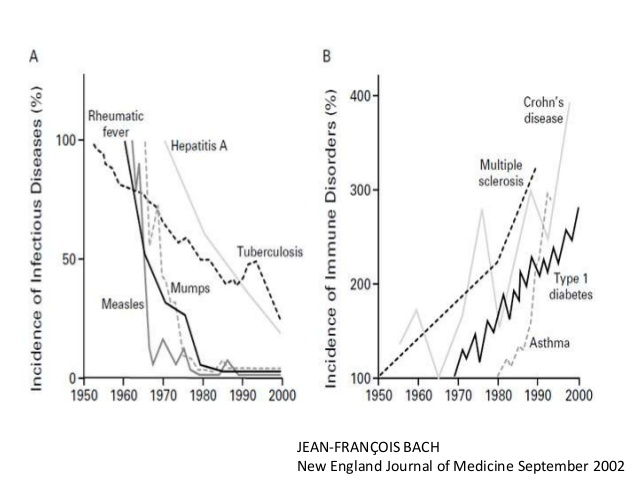
\includegraphics[scale=0.5]{img/allergie_infection.jpg}\hfill
\end{center}
\caption{Incidence des maladies infectieuses et autoimmune en europe au cours du temps}
\label{bach}
\end{figure}


Depuis peu, les nouvelles méthodes d'exploration de ce monde microscopique, comme le séquençage de l’ARN 16S a permis aux bactéries de retrouver leurs lettres de noblesse.
Les bactéries sont retrouvé partout et s'accaparent les premiers rôles dans le fonctionnement des écosystèmes. Elles sont par exemples impliqué dans le cycle de l'azote en permettant à la biomasse d'absorber l'azote athmosphérique. Les bactéries sont dans ce sens, la seul source d'azote permettant de construire nos protéines et notre ADN.
Elles peuvent vivre dans les milieu les plus inhospitaliers. Les archébactéries par exemple, peuvent résister à des conditions d'acidités et de températures exceptionnelles. On les retrouve dans les fonds océaniques, ou privé de lumière, elle sont la seul source d'énergie pour toutes la faune via la chimiosynthèse \footnote{La chimiosynthèse à l'instar de la photosyntèse produit de l'énérgie à partir d'une réaction de réduction du soufre}. C’est d’ailleurs leurs découverte qui nous a éclairé sur l’origine des eucaryotes \footnote{Le génome des archéobactéries est composé d'intron comme les eucaryotes} et qui nous a permis de faire un bon de géant en biologie moléculaire \footnote{La Taq polymérase est un enzyme d'archébactérie résistant à de haute temperature utilisé pour faire des PCR}.\\
L'homme ne fait pas exception. Les régions anatomiques autrefois considéré stérile foisonnent à présent de bactéries. En effet la majorité des bactéries ne poussant pas en culture, elle ont longtemps été indétectable. 
Elles sont retrouvé dans toutes les régions du corps exposés ou elles forment des communautés.
La peau est colonisé par \textit{Propionibacterium}, \textit{Corynebacterium} et \textit{Staphylococcus} \citep{Beck}. Le vagin contient les bacille de Döderlein et la bouche principalement du \textit{Streptococcus}\cite{Beck}.
L'intestin est une flore bactérienne dominé par les anaérobie et pouvant représenté jusqu'à 2 kg du poids corporel \citep{Beck}.
En échange de son hospitalité, le microbiote participe au bon fonctionnement de son hôte. Il aide à la digestion en dégradant par exemple les sucres du lait maternelle chez le nouveaux née[@bifidus]. Il participe à la synthèse de vitamine essentiel (K, B12,B8)[@ref]. Il éduque notre système immunitaire et fait barrières à tout nouvel agent pathogène.
Tout défaillance de notre microbiote ou \textit{dysbiose}, peut être délétère pour notre santé. La liste des maladies associés est longue. On retrouve par exemple la maladie de Crohn[@], la maladie coeliaque[@], le cancer de l’intestin[@], le syndrome du colon irritable[@], l’obésité[@], le diabète de type 1[@], l’asthme[@], l’eczéma[@], la sclérose en plaque[@], la polyarthrite rhumatoïde[@], la maladie d’alzheimer[@] et même l’autisme[@]. \\
La colite à \textit{Clostridium Difficile} est un exemple de dysbiose avec une application clinique directe. Suite à un traitement par antibiotique, la flore intestinale est détruite laissant alors l'oportunité à \textit{Clostridium Difficile} de s'installer. Un des traitements proposé est la transplantation fécale visant à réintroduire un microbiote au patient. \\
Le microbiote amène donc à reconsidérer notre individualité. Nous ne sommes pas qu’un eucaryotes multicellulaire composé d’un unique génome. Mais un écosystème ou cellules eucaryotes et microbienne vivent en symbiose. Cette relation n'étant pas figé dans le temps et pouvant varier entre le commensalisme, la parasitisme et le mutualisme. Les dernières études estiment que pour chaque individus il y a environs 30 billions de cellules humaines pour 39 billions de cellules microbiennes[@]. En associant les gènes bactériens, le génome d’un individu passe de 23 000 gènes à 3,3 millions[@] de gènes avec toutes la complexités des interactions que cela engendre.[@] Les scientifiques ont donnée le nom d’\textit{holobionte} à cette entité vivante hétérogène. Pour pousser le vis, l'ensemble du génome humain et microbiens est appelé \textit{hologénome} \footnote{Pour certain, l'hologénome est la cible de la sélection naturelle}. \\
Il faut tout fois rester prudent quant au rôle donné aux microbiotes et éviter de tomber dans excès. Nombreux sont les publications scientifiques qui se contredisent et qui ne montrent que des corrélations, sans rapport direct de causalité. Cette excès de publication à même conduit à la création du hashtag humouristique sur twitter: \textit{\#GutMicrobiomeAndRandomSomething} ou les gens publiaient les corrélations les plus absurde[@]. \\
En effet, l'hygiène n'est pas le seul facteur a avoir changer dans nos société. D'autre facteur, comme la sédentaire ou notre alimentation, peuvent tout aussi bien être impliqué dans la survenue de maladie.
Les études sur le microbiotes nécessitent d'être réalisé à plus grande échelle avec plus de patient et avec un suivi à long terme important. Les nouvelles technologies de séquençage haut débit vont dans ce sens en permettant de collecter des quantités de donnée impressionnante limité seulement par les capacités de calculs. \\
Il n’y a pas de honte à dire aujourd'hui, nous ne connaissons pas grand chose au sujet du microbiote humain. C’est une science naissante et seul le futur nous dira si il s’agit d’un effet de mode ou d’une révolution. \\
Au regard de la biologie évolutive, il y a fort à parier dessus. Car ne l'oublions pas, ce sont bien des anciennes bactéries, qui permette à l'ensemble de nos cellules de respirer et que nous appelons maintenant mitochondries.

\begin{figure}[ht]
\begin{center}
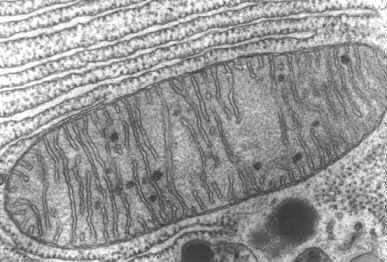
\includegraphics[scale=0.5]{img/mitochondrie.jpg}\hfill
\end{center}
\caption{La mitochondrie est l'exemple de symbiose ultime entre eucaryote et procaryote}
\label{bach}
\end{figure}



\newpage

\section{Définition}

\begin{description}
  \item[Le microbiote] est l’ensemble des micro-organismes (bactéries, levures, champignons, virus) vivant dans un environnement donné.
  
\item[Le microbiome] s’emploi selon deux définitions. En français, le microbiome est l'environnement qui héberge le microbiote. Dans sa définition angle-saxonne, le microbiome fait référence à l’ensemble des génomes microbien contenu dans un environnement. 
De façon général le microbiome est associé aux génomes bactériens. Les termes de Virome et de Mycobiome sont utilisé pour les génomes viraux et myoctiques. 

\item[La biocénose] est le terme écologique dans un sens large désignant l'ensemble ds organismes vivants dans un environnements appelé \textbf{Biotope}. Biocénose et biotope forme ensemble un \textbf{écosystème}.

\item[Une symbiose] est une association durable entre deux organismes. Leurs relations peuvent être mutualistes, parasitaire ou commensale.

\item[La métagénomique] est une méthode d’étude du contenu en ADN présent dans un milieu grâce au technique de séquençage haut débit. Contrairement à la génomique qui s’intéresse au génome d’un individu, la métagénomique s’intéresse aux génomes d’une population d’individu.
Dans son sens stricte, la méta-génomique correspond à l’étude de l’ensemble des séquences d’ADN. L’analyse d’un seul gène, comme celui de l’ARN 16s est associé à tord au terme métagénomique, mais son usage reste courrant. On lui préférera le terme de \textbf{metagénétique}

\item[Un read] est un terme bioinformatique désignant une séquence d’ADN issue d’un séquençage haut débit. Selon les technologies, les reads varient entre 150 et 300 paire de bases.

\item[Un OTU] (\textit{Operational taxonomic Init}), est un terme utilisé en phylogénie, désignant un groupe d’individu proche et fait souvent réference à l’espèce dans la classification de Linée.
En microbiologie, un OTU fait référence à un groupe d’individu ayant une similarité dans leurs séquence d'ARN 16s supérieur à 97\%

\item[L'Abondance] absolu est le nombre de séquences d’ADN d’un OTU retrouvé dans un échantillon. 
L’abondance relative est le pourcentage en séquences d'ADN d'un OTU retrouvé dans un échantillon. Ce dernier indicateur permet de rendre les échantillons comparable entre eux.


\item[La table des OTU] correspond à un tableau à double entrée contenant l’abondance d’un OTU pour chaque échantillon. Dans le tableau suivant, l'échantillon 1 contient 68\% de l'OTU 1.

\begin{figure}
\begin{center}
\begin{tabular}{|l|c|c|c|c}
  \hline
   & échantillon 1 & échantillon 2 & échantillon 3  \\
  \hline
  OTU 1 & 68\% & 12\% & 25\% \\
  OTU 2 & 40\% & 24\% & 25\% \\
  OTU 3 & 28\% & 64\% & 50\% \\

  \hline
\end{tabular}
\end{center}
\caption{La table des OTUs}
\end{figure}

\item[La diversité alpha] est une mesure de biodiversité au sein d’un échantillon. Elle correspond donc à l’étude d’une colonne dans la table des OTUs. Plusieurs indicateurs de diversité alpha.

\item[La diversité beta] est une analyse descriptive de la biodiversité entre plusieurs échantillons. Elle correspond à l’étude de l’ensemble de la table des OTUs. L’approche la plus courante est de réalisé une analyse multivarié par des méthodes d’ordination. Il s’agit de représenter un graphique à N dimensions, impossible à dessiner, en le projetant dans un espace à une ou deux dimensions.

\item[La richesse] est le nombre d’espèce présent dans un échantillon. Les deux échantillons suivant ont la même richesse de 2. 

échantillon 1  : 4 Streptoccus , 4 Escherichia  \\ 
échantillon 2 : 432 Streptoccus, 12 Escherichia 

\item[L'uniformité] indique si les espèces d’un échantillon sont répartis uniformément.
L'uniformité du premier échantillon est plus grand que le second

échantillon 1  : 50 Streptoccus , 50 Escherichia  \\ 
échantillon 2 : 432 Streptoccus, 12 Escherichia 


\item[L'indice Chao1] est une estimation de la richesse réel (in vivo) par rapport à la richesse observé (in vitro). Cette indice part du principe que si l’échantillon contient beaucoup de singletons ( OTU détecté une seul fois), il est fort probable que la richesse réel soit plus grande que la richesse de l’échantillon. La formule est la suivante.
\begin{equation}
\end{equation}

\item[L'indice de Shannon] est un indicateur évaluant à la fois la richesse et l’uniformité dans un échantillon. Il se calcul de la même façon que l’entropie de shannon.

\begin{equation}
\end{equation}

\item[L'indice de Shannon] est un indicateur évaluant la probabilité que deux individus sélectionnées aléatoirement dans un échantillons donnée soient de la même espèces. La formule est la suivante.

\item[Pipeline] 
Il s'agit d'un outil informatique permettant de distribuer les différentes operations de calcul sur plusieurs processeurs en même temps. Pour illustrer ces propos, imaginons qu’un pipeline est une recette de cuisine, composé de plusieurs étapes successif. Sans parallélisation, un cuisinier doit attendre que chaque étape se termine avant de passer à la suivante. Faire fondre le beurre, puis dans un second temps battre les oeufs en neige ( Exécution synchrone). En parallélisant, le cuisinier peut faire plusieurs étapes en même temps. Battre les oeufs pendant que le beurre fondent. ( Exécution asynchrone). Maintenant, si l’on demande à 40 cuisiniers ( processeurs) de faire 188 gateaux, l’organisation des tâches devient complexe si l’on veut distribuer toutes les tâches de façon à maximiser les performances.

\item[La courbe de rarefaction] est utilisé pour determiner si la profondeur de séquençage est suffisante pour caracterisé la diversité d’un échantillon.
Pour génerer cette courbe, des groupes de reads de taille croissante (1…n) sont tiré aléatoirement sans remise. Pour chaque groupe en absisse le nombre d’OTU correspondant est reporté sur l’axe Y.
Une courbe s’applatissant indique qu’une profondeur de séquençage plus grande, n’apporterai pas plus d’information. \citep{Dickson2014} and \citep{Beck}

\end{description}

\setcounter{page}{1}

\section{Introduction}
\subsection{La mucovicidose}
\subsubsection{Une maladie génétique}
La mucovicidose est une maladie génétique autosomique recessive grave touchant en france 1 naissance sur 5400 [@]. La bretagne est la région la plus touché avec une prévalence de 1/3000[@].
La loi de Hardy Weinberg estime qu’en bretagne 1 patient sur 25 est porteur de la mutation à l’état hétérozygotes[@Heterozygote advantage]. Cette haute prévalence s’explique probablement par un effet fondateur associé à un avantage séléctif pour les individus porteur de l’allèle muté. \footnote{Plusieurs hypothèses ont été proposé, notamment lors des grandes épidémies de choléra en diminuant les pertes hydriques. D’autres suggère qu'il s'agit d'une pleiotropie antagoniste.[@]} \\
Le gène CFTR impacté se situe sur le chromosome 7 en position q31.2. Il est constitué de 27 exons pour 250,188 [@] paire de bases. Il code pour une canaux chlore AMp dépendant permettant les échanges des ions chlorures au niveau des membranes cellulaire.[@]. Il est également impliqué dans le transport du thiocynate (SCN-) et des bicarbonate (HCO3-).[@]. \\
On dénombre à ce jour 2017 mutations impliquées dans la mucovicidoses[@]. La perte d’une phénylanine en position 508 par délétion du triplet c.1521-1523delCTT (anciennement $\Delta$F508) est responsable à elle seul de 80\% des mucovicidoses.
Ces mutation peuvent être responsable d’une protéine défectueuse ou d’une absence de canaux sur les membranes cellulaires. \\
Cliniquement, la mutation est responsable chez les patients d’une insuffisance pancréatique exocrine et d’une infertilité par disparition des canaux déférant. Des signes digestif, hépatique et articulaire sont également retrouvés.
L'atteinte de la fonction réspiratoire est la plus bruyante. En effet au niveau de l’epithélium broncho-pulmonaire, l’absence d’un CFTR fonctionnelle est à l’origine d’une desyhdration du mucus le rendant plus visceux et empêche les cils bronchiques de jouer leurs role.[@]\\
La forte prévalence de la maladie nécessite de réaliser un dépistage précoce chez tous les nouveaux née (test de Gutri) afin d’adapter au plus tôt la prise en charge. Seul le test à la sueur permet de poser le diagnostic. Des test de dépistage prénatal basé sur l’ADN circulant sont actuellement à l’étude. Le traitement repose avant tout sur une prise en charge réspiratoire (kinésithérapie, dornase, antibiothérapie).
Les thérapies génétiques sont encore à l’étude[has]
L’Ivacaftor est le seul traitement à ce jour qui agit directement sur le CFTR. Maise concerne uniquement certaine mutation, comme la G551D.[has]La greffe pulmonaire est le dernière recours.

\subsubsection{Une maladie infectieuse}

L’atteinte pulmonaire est caractérisé par des infections successive associé à une réaction inflammatoire qui dégrade progressivement la fonction réspiratoire.
Plusieurs pathogènes sont impliqué. Chez les jeunes enfant, \textit{Haemophilus influenza} et \textit{Staphilococcus Aureus} sont majoritairement retrouvé. \textit{Burkolderia Cepace} et \textit{Stenotrophomonas Maltophilia} sont retrouvé chez le sujet plus agé.
Mais c’est \textit{Pseudomonas Aeruginosa} qui caractérise l’atteinte pulmonaire dans la mucovicidose en marquant un tournant décisive dans l’évolution de la maladie. Ce bacille aérobie strictes, est un germe de l'environnement rarement retrouvé chez les patients sains[@]. En revanche il est retrouvé chez 60\%[@] des patients jeunes, et plus de 90\% des patients adulte[@].\\
La primocolonisation à \textit{Pseudomnas Aeruginosa} est difficilement detectable, mais semble avoir lieu tôt dans l’enfance[@]. Il y a ensuite une phase de latence, variable entre individus, marqué par des épisodes d’exacerbations. A ce moment l’éradiction[@] par des antibiotiques reste possible.
Puis survient le passage à la chronicité. \textit{Pseudomnas Aeruginosa} s'adapte à son milieu et s’installe à long terme. Il perd certain caractère de virulence, mais devient résistant au antibiotiques[@]. Son phénotype change. Il devient mucoïde en sécretant un film d’alginate qui le protège du système immunitaire. Les mécanismes sous jacent à cette transformation sont ingenieux. La forte densité en bactérie est résponsable d’activation de certain gène amenant au phénotype mucoïde par un processus appelé \textit{quorum sensing}[@]. un processus dans lequel chaque bactéries communique avec ses voisins via des signaux\footnote{On peut comparé ce processus à un système multiagent. comme un banc de poisson ou le comportement global dépend du comportement d’un individu}.
Les génomes de \textit{Pseudomnas Aeruginosa} deviennent aussi hypermutable afin de présenter une plus grande diversité génétique au regard de la sélection naturelle\footnote{En biologie évolutif, il s'agit d'évolvabilité}. \\
A ce stade le traitement antibiotique n’est plus curatif et l'evolution tend inexorablement vers un déclin de la fonction respiratoire.
L'approche clinique est donc préventif. Elle  vise à éliminer \textit{Pseudomnas Aeruginosa} dès qu’il est détecté en culture. Une surveillance rapproché des patients avec un prélevement mensuel ou bimensuel est préconisé. La culture étant peu sensible, d���autres méthode détection peuvent être employé. La détection des anticorps anti-pyocianique par des méthodes elisa a montrer peu de …[]
La PCR ciblé associant les protéines bactériennes \textit{OPRL1} , \textit{GYRB1} et \textit{ECFX1}  s’est montré plus sensible et plus spécifique que la culture[@]. \\
En pratique, la colonisation chronique est défini lorsque 3 expectorations sont rendu positif en culture, successivement au cours d’un suivi mensuelle ou bimensuel[@].
Une autre classification, celle de Lee a montrer une forte liaison clinico-biologique. Elle est composé de 4 groupes :  
\begin{description}
\item[groupe chronique] > 50\% des cultures sont positives sur 12 mois
\item[groupe intermediaire] $\leq$ 50\% des cultures sont positives sur  12 mois
\item[groupe Free] Toutes culture négative sur 12 mois, avec des antécédants
\item[groupe Never] Toutes culture négative sur 12 mois sans antécédants 
\end{description}

On ne sait pas aujourd’hui pourquoi \textit{Pseudomnas Aeruginosa} s’installe préférentiellement chez les patients atteind de mucoviscidoses. Plusieurs hypothèse ont été posé : 

\begin{itemize}
\item La dysfonction cilliaire empêche les Pseudo d’etre viré
\item L’hypersalinité du film muqueus desactive les peptides antimicrobien
\item Le CFTR est un recepteur de Pyo pour les internalisé et les viré
\item L’inflammation de de l’eopthelium augmente les metabolite qui permette de se developper.
\item Alanine et lactta sont une source de carbonne pour le Pyo.
\item Le microbiote influence la colonisation
\end{itemize}




\begin{figure}[ht]
\begin{center}
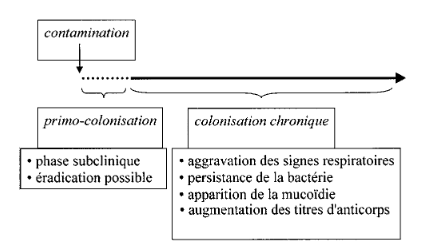
\includegraphics[scale=0.8]{img/chronic.png}\hfill
\end{center}
\caption{Infection pulmonaire à pyo dans la mucovicidose. ref []}
\label{bach}
\end{figure}


\subsection{Le microbiote pulmonaire}

Bien qu’il soit en contacte avec le milieu exterieur, l’arbre réspiratoire (comprenant la traché, les bronches et les alvéole) a longtemps été considéré comme stérile avec les méthodes de culture classique. Il a fallu attendre l’avenement du séquençage haut débit pour mettre en évidence le microbiote pulmonaire[ref Host-microorganism 1-3].
Le microbiote pulmonaire, est beaucoup moins abondante que la flore digestif. Il est constituté d’une flore dynamique provenant essentiellement de l’air ambiant mais aussi du tube digestif via des microaspirations.[@]
Le microbiote pulmonaire est dominée par le phylum des Firmicutes ( Streotpococcus) et des Bacteroidetes (Prevotella).[pie] Les genres retrouvé majoritairement sont Streptococcus, Prevotella, Fusobacteria, VBeillonella, Haemophilus, Neisseria et Porphyromonas.
l’arbre réspiratoire étant en continuité direct avec les voies aérienne superieur, certain genre bactérien sont commun, comme Streptococcus, staph, Haemophilus et Moraxella. Tandis que d’autre genre comme corynebacterium et Dolosigranulum ne sont retrouvé qu’au niveau des voies aérienne superieur.

Le microbiote varie dans l’espace et le temps. \\
Dans l’espace, du fait de sa structure, certaine régions de l'arbre bronchique peuvent présenter des microbiote différent. Un prélèvement d'un foyer infectieux sera nécessairement différent d'un foyer sain. Le poumons présente également des différences physicochimiques selon la localisation pouvant selectionner certaine espèces. Les cavernes tuberculeuses par exemple, se trouve essentiellement dans le lobe supérieur en raison d'une concentration en oxygène plus élevé favorisant ce bacille aérobie stricte. (anaeobie stricte, et pas d’autre?)\\\
Le microbiote varie dans le temps.... 
Plusieurs études suggère une différence de microbiote entre patient sains et avec une atteinte réspiratoire chronique comme l’asthme, la BPCO et la mucovicidose [ Huang et all 2010].
Plusieurs études suggère que certain microbiote sont associé à des pathologies comme l’asthme, la BPCO ou la mucovicidose. Le mécanisme sous jacent, théorie hygieniste, stipule que les bactéries stimule le Systeme immunitaire.
propre a chaques individus
variable dans le temps
variable selon les localisation
résilience des population
les résident peramanent et les attack
Liens avec les maladies :
– hygeniste

\subsection{Exploration du microbiote pulmonaire}
%(http://bacterioweb.univ-fcomte.fr/bibliotheque/remic/08-Bronc.pdf) ==> A LIRE COOURS BACTERIO
Le microbiote pulmonaire est explorer par le séquençage des ADNs bactériens présent dans un prélevement broncho-pulmonaire. Toutes les méthodes de recceuils sont possible, mais les prélevement protégé sont recommandé afin d’éviter une contamination par les voies superieurs.
Après extraction de l'ADN, 2 strategies de séquençages peuvent être employé: \\
Le stratégie shotgun consiste à séquencer l'ensemble des ADNs présents dans l'échantillon sans discernement. Les séquences sont filtrer puis les génomes bactériens sont reconstruit par des méthodes bioinformatiques complexes. \\
La deuxième stratégie est moins couteuse en terme d'analyse. Elle consiste à amplifier un gène assez variable pour pouvoir discriminer une espèces. Pour les bactérie il s'agit de l'ARN 16S. Il s'agit d'un ARN non codant participant à la structure de la petite sous unité des ribosomes bactériens. Il est composé de 1500 nucléotides et forment plusieurs boucles dans sa structures secondaires (Figure \ref{ARN16S}). 
L'alignement des séquences d'ARN 16S entre plusieurs espèces met en évidence des régions constantes et variables Figure \ref{ARN16SVariation}). Les 9 régions variables appelé V1 à V9 peuvent être amplifié puis séquencer afin d'identifié l'espèce correspondante.

\begin{figure}[ht]
\begin{center}
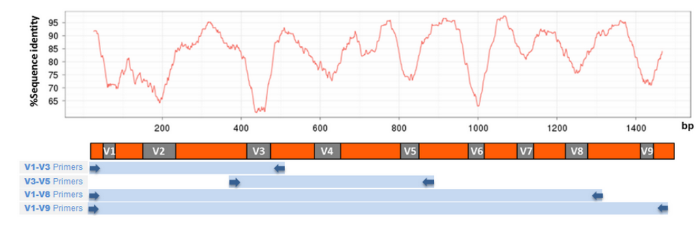
\includegraphics[scale=0.8]{img/ARN16S_variation.png}\hfill
\end{center}
\caption{région constante et variable de l'ARN 16S}
\label{ARN16SVariation}
\end{figure}

\begin{figure}[ht]
\begin{center}
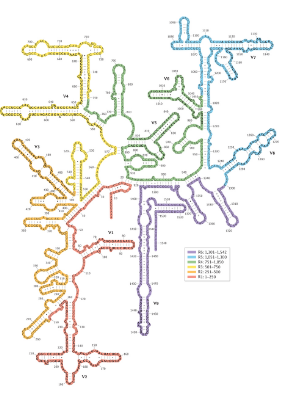
\includegraphics[scale=0.8]{img/ARN_16S.png}\hfill
\end{center}
\caption{Structure secondaire de l'ARN 16S}
\label{ARN16S}
\end{figure}


La première stratégie est plus informatif car elle séquence l'ensemble des génomes bactérien et permet de prédire la fonction d'un microbiote. En effet les transfert génétique horizontaux amènent à dissocié l'espèce de sa fonction. 2 bactéries d'une même espèce peuvent avoir des fonctions différentes. L'inférence fonctionnelle réalisé à partir du taxon bactérien est déconseillé.  
La stratégie 16S reste une méthode simple pour décrire les populations bactériennes présentent. C'est cette dernière qui a été employé dans notre étude. 


\subsection{Objectif de l'étude Mucobiome}
L'objectif de notre étude est de savoir si le microbiote réspiratoire influence la primocolonisation à \textit{Pseudomnas Aeruginosa}. 
Pour cela, nous avons suivit pendant 3 ans,  une cohorte de 47 patients atteints de mucovicidoses sans infection chroniques. 
L'exploration de leurs microbiote par la stratégie 16S a été réalisé sur leurs ECBC dans le cadre de leurs suivi régulier. 
A partir des données généré du séquençage, nous avons réalisé l'étude descriptive et analytique de leurs microbiotes en créant un pipeline bioinformatique dédié. 

\section{Materiel et Méthodes}
\subsection{Recueil des données}

47 patients atteind de mucovicidoses ont été suivit sur 3 ans ( 2008-2011) dans une étude prospective multicentrique (Nantes,Brest,Roskoff) appelé mucobiome.
Les dates de prélevement sont illustré dans la figure x.
La CPP VI-Ouest et le commité d’éthique du CHRU de Brest ont approuvé le protocole. Tous les patients ( ou les parents pour les mineurs) ont signé un consentement éclairé. Le protocole à fait l’objet d’une déclaration de biocollection à l’ARS et au MESR (n DC-2008-214).\\
les ECBC des patients ont été receuillies lors des séances de kinésithérapie réspiratoire tous les 3 mois, suivant le calendrier des recommandations officielles. En pratique, sur l’ensemble de la cohorte suivie, l’intervalle median entre 2 consultations a été de 3.4 mois.
Les patients devaient avoir un genotypage CFTR et un test à la sueur positif. Les transplanté ont été exclus de l’études.
Une culture positive à \textit{Pseudomnas Aeruginosa} était un critère de non-inclusion. Si pendant l’étude, une culture revenait positif à ce dernier, le patient était sortie de l’étude pour être réinclus 1 ans après en l’absence de colonisation chronique. 15 patients ont été ainsi réinclus.
Chaque patient a été classé dans la categorie Free ou Never (Lee et all 2003). D’autres données ont été également recceuilli ( tableau).
Au total , 188 échantillons ont été récolté, soit en moyenne 4 échantillons par patients.
Pour chaque échantillon, une culture a été réalisé en suivant les procédure standard [ref]. Une qPCR ciblant le \textit{Pseudomnas Aeruginosa} a également été réalisé en combiant les marqueurs gyrB/ecfX designé au laboratoire[ref].

\subsection{Extraction de l’ADN}

Les échantillons ont été liquéfié avec du Dithiotrétiol . Les protéines ont été degrédé avec une Proteine kinase.
Les parois bactériennes ont été fragmenté par sonication. (DTTpar sonication (Elamsonic S10, Singen, Germany). Après 10 min de centrifugation, L’ADN a été extrait à partir du culot via QUIAamp DNA Minikit ( Quagen).
Les extraits d’ADN ont été envoyé pour séquençage via un prestataire GATC.

\subsection{Séquençage}
La librarie \footnote{l'ensemble des fragments d'ADN à séquencer} a été produit en amplifiant la région V3-V5 à l’aide du couple d’amorces  \textit{forward(CCTACGGGAGGCAGCAG)} et \textit{reverse(CCGTCAATTCMTTTRAGT)} et du kit MiSeq Reagent Kits v3. \\
La séquençage a été produit sur Illumina MiSeq. Cette technologie permet de lire deux séquences de 300pb d'un fragment d'ADN par ses deux extrémités. La figure \ref{illumina} montre le chevauchement de ces deux reads pairés qui permet de lire l'amplicon V3-V5 de 535pb. \\
Environ 25 millions de reads sont produit par run. En multiplexant à l’aide de 94 index, 2 runs ont permis de séquencer les 188 échantillons.
Au final 188 x 2 fichiers fastq ont été généré à l’issue du séquençage.

\begin{figure}[ht]
\begin{center}
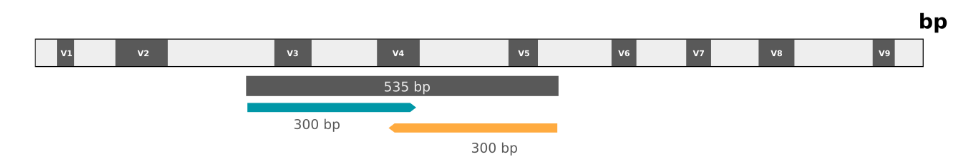
\includegraphics[scale=0.6]{img/illumina.png}\hfill
\end{center}
\caption{le couple de séquence de 300pb permet de recouvrir l'ensemble de la région V3-V5}
\label{illumina}
\end{figure}


\subsection{Analyse bioinformatique}

l’analyse des 188 x 2 fichiers fastq a été réalisé grâce à un pipeline bioinformatique, appelé \textit{mucobiome}, conçu et tester dans le cadre de cette étude. Par rapport aux autres logiciels comme \textbf{QIIME} ou \textbf{MOTHUR}, le pipeline mucobiome est spécialisé dans l’analyse des données 16S. Il est également plus rapide en raison d’un très haut niveau de parallélisation permis grâce à  \textbf{Snakemake}. Cette outil modélise l'ensemble du pipeline sous forme d'un graphe direct acyclique (DAG) et le résoud afin d'optimiser le parallélisation. \\
Le pipeline mucobiome prend en entrée, les 188 fichiers fastq provenant du séquençage et produit un fichier BIOM contenant la table des OTUs.

FIGURE SIMPLE

\begin{figure}[ht]
\begin{center}
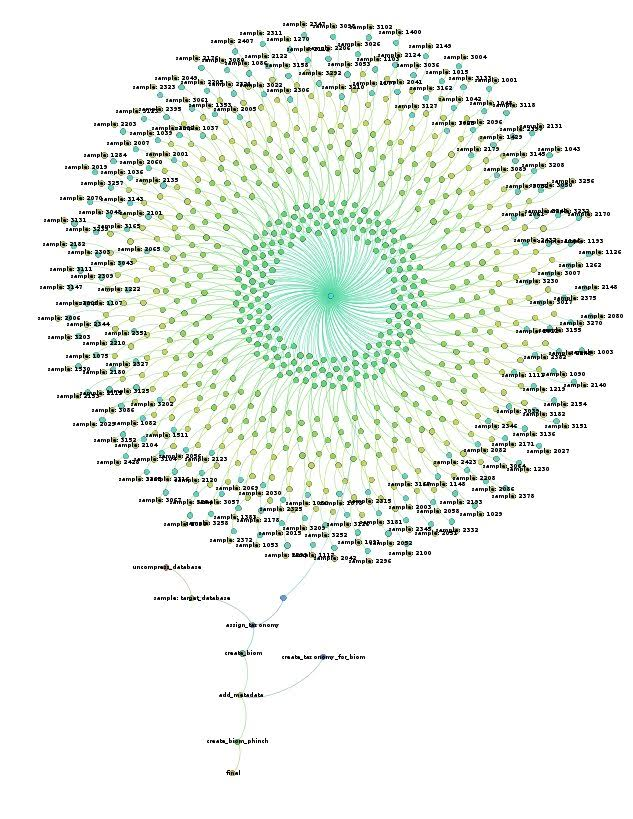
\includegraphics[scale=0.4]{img/dag.jpg}\hfill
\end{center}
\caption{le graph du pipeline sur les 188 échantillons}
\label{dag}
\end{figure}


\subsubsection{Pré-Traitement}

\subsubsection{Verification des qualités}

\subsubsection{Fusions des reads}

Les données bruts provenant d’un séquenceur sont des fichiers FastQ ( annexe ). Ces fichiers contiennent les séquences nucléotidique et les scores de qualités de l’ensemble des reads lu par le séquenceur. La stratégie de séquençage étant paired-end, pour chaque échantillon séquencé, deux fichiers fastq sont fourni. L’un correspond à la séquence lu dans le sens forward et l’autre lu dans le sens reverse.
La première étape du pipeline consiste donc à fusionner ces deux fichiers . c’est à dire fusionner les reads deux à deux afin de produire un plus long reads de 500 pb en moyenne. Cette plus longue séquence correspond à la région V3-V5 de l’ARN 16S.
2 algorithmes ont été utilisé pour la fusion des reads, et sont mis à disposition de l’utilisateur.

Flash

VSearch

\subsubsection{Trimming des reads}

Afin d’assurer un alignement parfait, les séquences ne contenant pas à leurs extremités les amorces V3-V4 ont été supprimées ou ajuster.
L’algorithme utilisé est celui de cutadapts. Cette algorithmes reconnait avec un tolérence ajustable ( 0.1 par default) les amorces puis ajuste le reads en retirant les nucléotides en excès. Lorsqu’aucune séquences d’amorces n’est retrouvé, le read est supprimé .

\subsubsection{Filtrage des qualités}

Les données provenant de séquenceur haut débit peuvent contenir de nombreuses erreurs de séquençage comparé au méthode classique comme la méthode Sanger. Ceci est particulièrement vrai avec la stratégie MiSeq et le kit 300pb. Il est donc important de supprimer les reads de mauvaise qualité pour gagner en spécificité.
Tout d’abord une analyse évaluant la qualité des reads à été réalisé sur chaque échantillon avec le logiciel FastQC. Ce programme produit à partir des fichiers fastq une série de graphiques permettant de juger sur la qualité du séquençage.
Après cette analyse, le filtrage des reads de mauvaise qualité est exécuté en utilisant le programme sickle. L’alogirthme sous jacent repose sur une fenêtre glissante de taille défini ( par defaut : 20 pb) qui glisse tout le long de la séquence. A chaque étape la moyenne des scores de qualité est calculé dans cette fenêtre. Si successivement le score moyen dépasse un certain seuil, le reads est supprimé . Par default le seuil utilisé est de 20 avec une fenêtre glissante de x.
Enfin FastQC a de nouveau été lancé afin de comparer la qualité des reads avant et après filtrage.

\subsubsection{Assignement taxonomique}

L’assignement taxonomique consiste à labelliser chaque reads à son taxon. Pour cela deux stratégies existent.
La stratégie “de novo” consiste à regrouper les reads qui se ressemble en groupe ou cluster.
Chaque cluster définit alors une seul séquence consensus qui est comparé à une base de donnée d’ARN 16S pour recevoir son assignation taxonomique.
La stratégie “close reference” consiste à labélisé chaque reads en les comparant directement un par un à une base de donnée. Cette dernière stratégie peut sembler plus longue, mais elle est en réalité beaucoup plus rapide que la première stratégie. En effet la compléxité de la stratégie “de novo” est de type N ( N le nombre de reads) . Chaque reads étant comparé à l’ensemble des reads le temps de calcul augment de façon exponnentiel avec le nombre de reads.
La complexité de la deuxième stratégie est elle de type N. C’est à dire que le temps de calcul augmente avec le nombre de reads de façon linéaire. En contrepartie, si un read n’est pas retrouvé dans la base de donnée, celui ci est ignoré. Alors qu’en stratégie “de novo”, tous les reads herite du taxon de leurs clusters.
Les bactéries de la flores humaines étant plus étudié que d’autre flore plus exotique, elle sont très souvent retrouvé dans les bases de donnée. La stratégie close réference est donc suffisante dans le cas de notre étude avec des testes préliminiares montrant une assignation reussi chez plus de 98% des reads.$

\subsubsection{Analyse descriptive}
L'analyse descriptif des données a été réalisé dans un script R. Les mesures d'alpha et de béta diversité ont été calculé avec le package phyloseq et les graphiques généré avec le package ggplot2. 
Le code source est disponible sur .... 

\section{Résultat}
\subsection{Pipeline Mucobiome}
Après demultiplexage, 188 x 2 fichiers fastq ont été généré soit 2 fichiers pairé par échantillons.
La taille des reads pour chaque fichier est de 301 paires de bases.
Au total 115’002’297 reads ont été produit sur 2 run MiSeq. Avec en moyenne 616900 reads par échantillon. Un minimum de 61422 reads pour l’echantillons 2154 et un maximum de 1071188 pour l’échantillon 3165.
Les analyses de qualité avec Fastqt montre dans l’ensemble une baisse de qualité en fin de séquence. Les 50 dernières bases, ont des scores de qualités médiocre entre 10 et 20 point selon le phred score.
Après prés traitement des reads, c’est à dire merging Flash et filtering 20, en moyenne 49.24 % des reads sont conservé avec des bornes allant de 37.30% à 61.13%.
L’assignement taxonomique a réussi sur 99.88% des reads.
Au total , le pipeline mucobiome s’est executé en 1h29 sur 40 coeurs et 20 giga de mémoire contre 42h dans les testes précédant sans optimisation.

\begin{figure}[ht]
\begin{center}
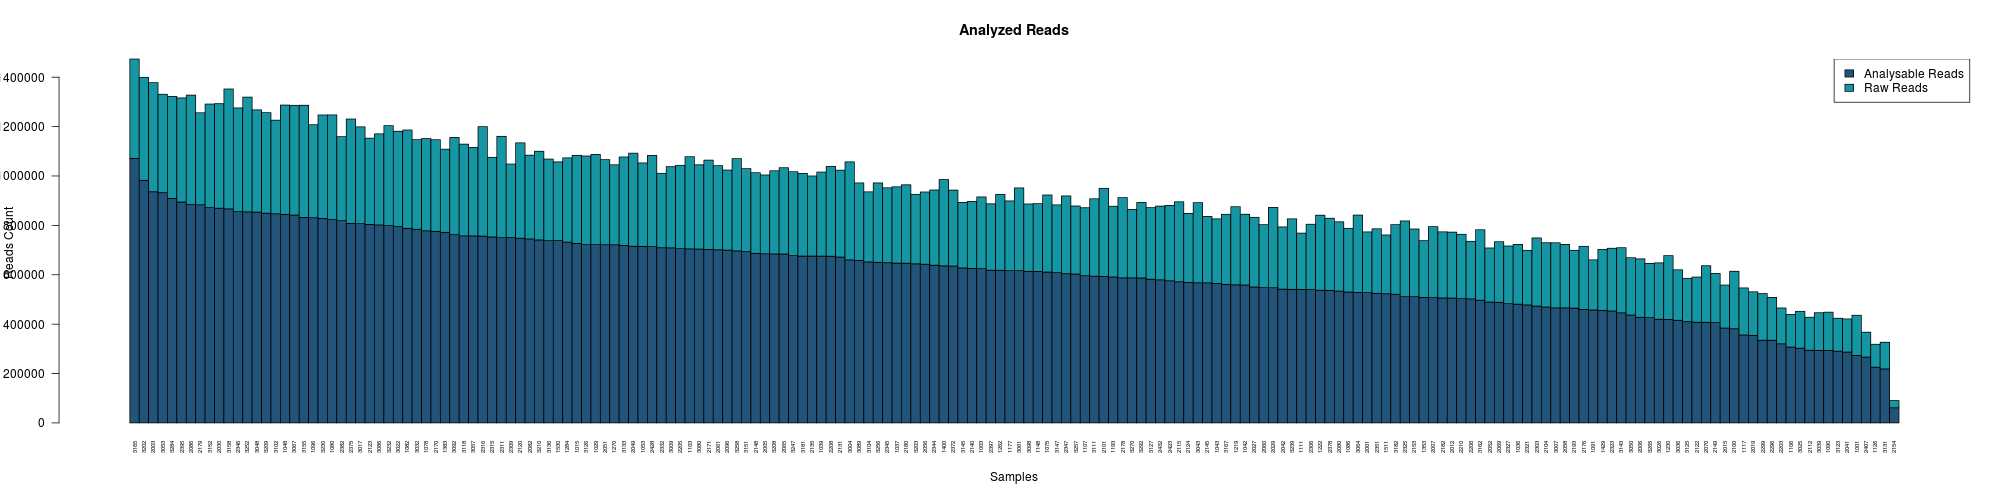
\includegraphics[scale=0.25]{img/pipeline.png}\hfill
\end{center}
\caption{Nombre de reads analysables avant et après filtrage}
\label{all}
\end{figure}




\subsection{Diversité du microbiote réspiratoire}

\subsubsection{Courbe de rarefaction}


\begin{figure}[!ht]
\begin{center}
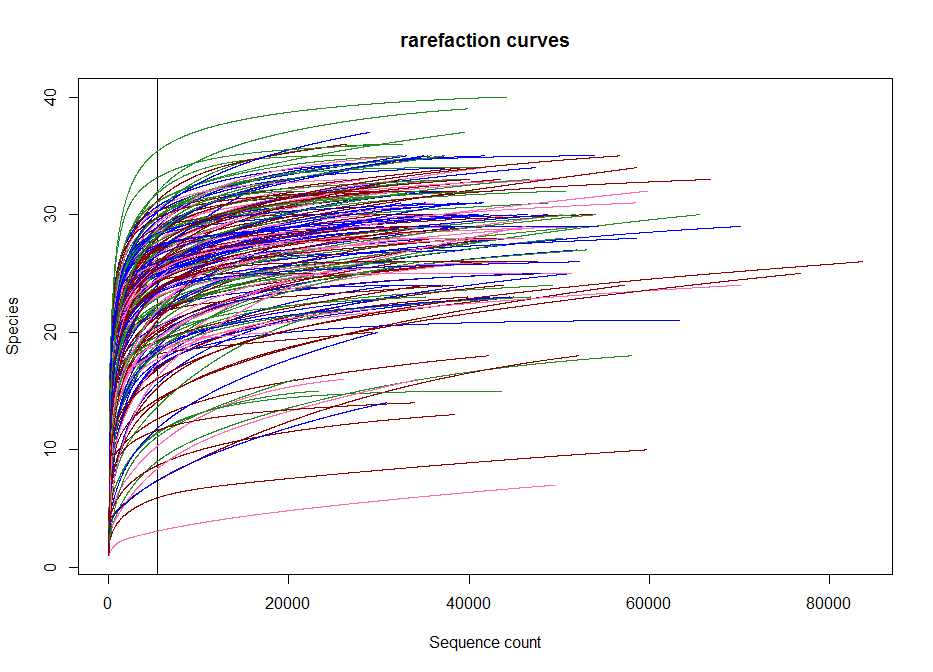
\includegraphics[scale=0.5]{img/rarefaction.png}\hfill
\end{center}
\caption{truc}
\label{bach}
\end{figure}




Les courbes de rarefaction par échantillons [figure] s’aplatisse précocement, témoignant d’un très bon niveau d’échantillonage.

\subsubsection{Diversité des échantillons}

Au total, 54 genres bactériens sont retrouvé dans l’ensemble des échantillons. [figure].
Les trois philums majoritaire, sont Protéobacteria(Haemophilus), Firmicutes(streptococcus) et Bacteroidete (prévotella). [figure pie].
Certaines genre bactérien sont très prévalente, c’est à dire présent dans l’ensemble des échantillons. Streptococcus, Neisseria, Prevotella, Granulicatella, Gemella, Veillonella et Fusobacterium sont présent dans plus de 185 échantillons.
D’autre sont dominante, c’est à dire qu’ils represente plus de 90% du microbiote pulmonaire dans certain échantillons. Il s’agit de streptococcus, Neisseria, Haemophilus et staphyloccoccus dans la majorité des cas. Sténotrophomonas et Achromobacter sont retrouvé dominante dans seulement 64 et 8 échantillons.
Le core microbiota est définit comme l’ensemble des taxons retrouvé dans plus de 50% des échantillons et ayant une abondance > 0.1%. Il est constitué de 15 genres décrit dans la figure [X].
La figure [violon] montre que Neisseria et Streptoccocus ont des abondances très variables dans les échantillons. Staphiloccocus et Haemophilus ont dans la plus part des échantillons des abondances relativement faible, mais la variance est tiré vers le haut par qque échantillons ou ils sont en dominance.


\begin{figure}[!ht]
\begin{center}
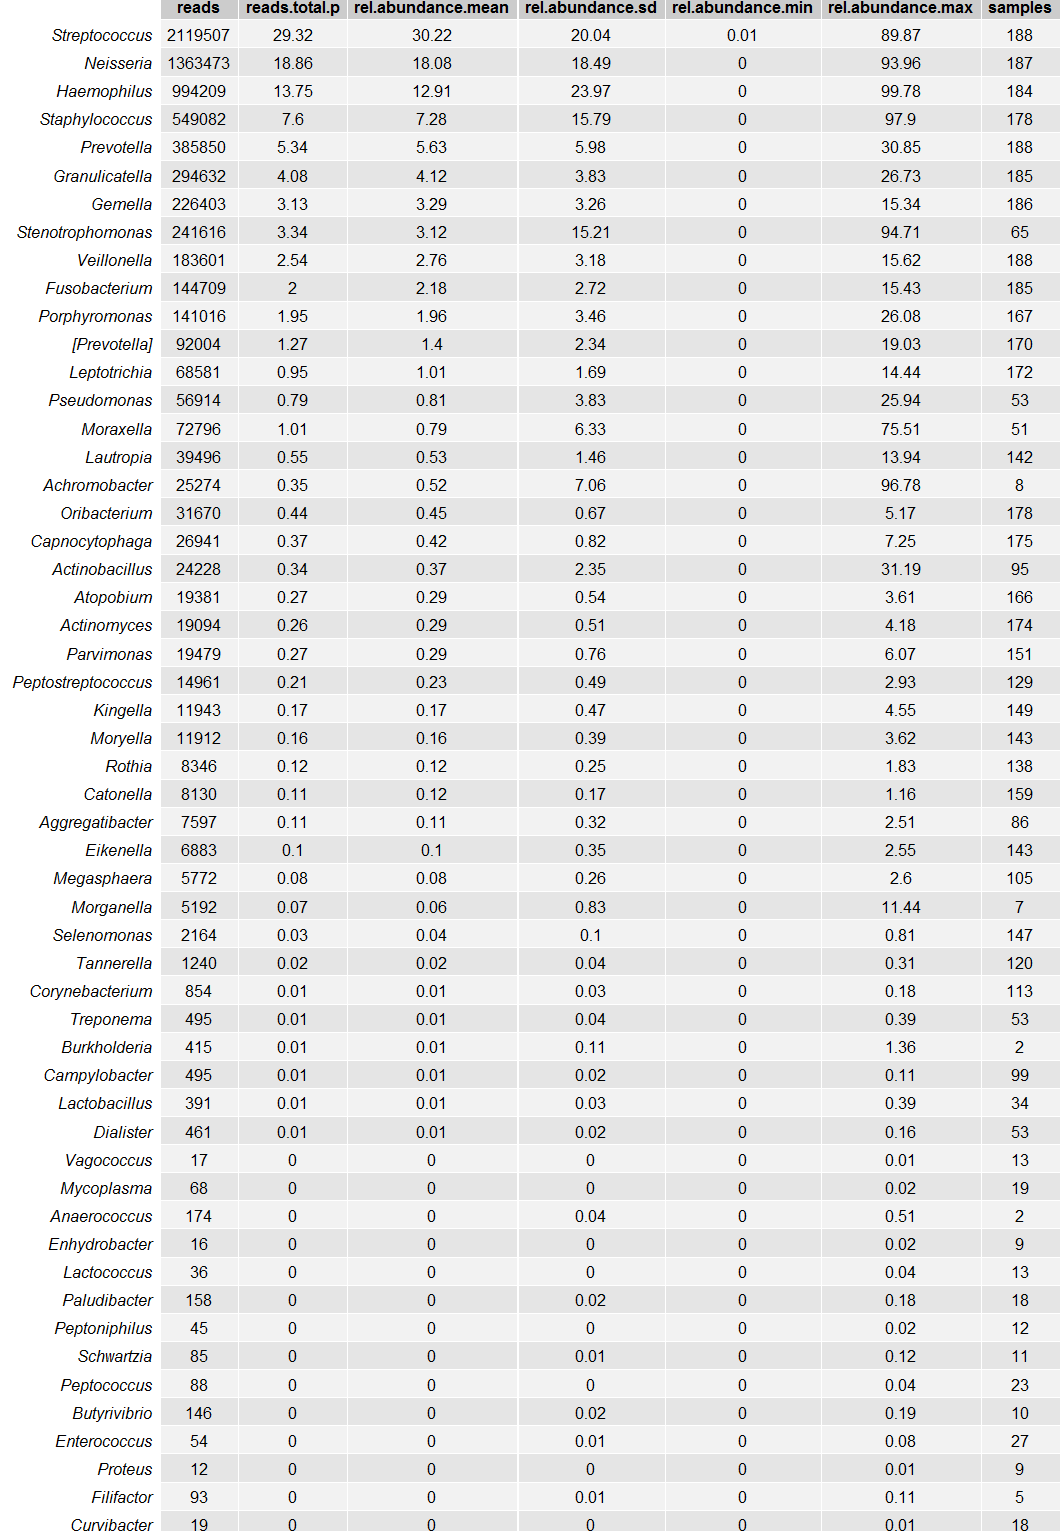
\includegraphics[scale=0.5]{img/all_table.png}\hfill
\end{center}
\caption{truc}
\label{bach}
\end{figure}






\subsection{Evolution dans le temps}
Alpha diversité (dot)
Abundance relatif (boxplot)
Alpha diversité (dot)
Abundance relatif (boxplot)Alpha diversité (dot)

\subsection{Comparaison entre catégories Free et Never}

\subsection{Sensibilité et Specificté du Pyo}

\section{Discussion}


\section{Conclusion}





\newpage

\appendix

\newpage


\bibliographystyle{plain}
\bibliography{biblio}

\end{document}
